\section{Introduction}\label{sec:intro}

\subsection{The moving sofa problem}

Let $L$ be the L-shaped hallway of unit width, the union of the horizontal side
$H_L=(-\infty,1]\times[0,1]$ and the vertical side $V_L=[0,1]\times(-\infty,1]$. A \emph{moving sofa} is a
closed connected planar set that can be moved rigidly from the horizontal side to the vertical side without
leaving $L$ (\cref{def:sofa}). Moser~\cite{Moser66} asked for the largest area of a moving sofa. The unit
square is a moving sofa of area $1$. Hammersley~\cite{Hammersley68} found a sofa of area $\pi/2+2/\pi=2.2074\ldots$, and
Gerver~\cite{Gerver92} one of area $2.21953\ldots$, bounded by 18 analytic arcs and segments, which he
conjectured to be optimal. Romik~\cite{Romik18} derived Gerver's sofa $\Gs$ from differential equations that
express the local optimality of its sides, and described its boundary explicitly in terms of two angles that solve
transcendental equations (\cref{fig:intro}, Appendix~\ref{app:gerver}). Kallus and Romik~\cite{KallusRomik18} proved by a computer-assisted method that no sofa has
area more than $2.37$. Baek~\cite{Baek} proved Gerver's conjecture in a paper of 119 pages: every moving
sofa has area at most $\abs\Gs=2.2195\ldots$.

\begin{figure}[ht]
\centering
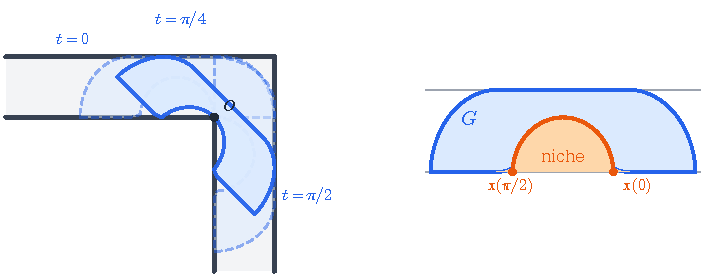
\includegraphics[width=\linewidth]{figures/fig-intro}
\caption{Gerver's sofa $\Gs$ in the hallway $L$. Left: it slides along the horizontal side (dashed), turns
through a right angle around the inner corner (solid, halfway, turned by $\pi/4$) and leaves along the
vertical side (dashed). Right: $\Gs$ with its niche, the hollow in its lower side that makes room for the
corner; the path $\xx$ of the inner corner of the hallway, as seen from the sofa, is drawn in orange.}
\label{fig:intro}
\end{figure}

\subsection{Uniqueness}

We prove that Gerver's sofa is the only optimal sofa, up to a rotation and a translation.

\begin{theorem}[uniqueness of Gerver's sofa]\label{thm:main}
Let $S$ be a moving sofa with $\abs S=\abs\Gs$. Then there are an angle $\theta$ and a vector $v$ such that
\[
  R_\theta S+v=\Gs .
\]
\end{theorem}

Equivalently, a moving sofa has maximum area if and only if it is a rotated and translated copy of $\Gs$
(\cref{cor:all}).

The theorem gives an equality of sets. This uses that a moving sofa is closed and that $\Gs$ is the closure of
its interior (\cref{sec:recovery}); equality of areas alone would determine a set only up to a null set.

The rotation in \cref{thm:main} can be taken to be trivial. The width of $\Gs$ exceeds one in every
direction other than the vertical (\cref{lem:gerver-width}), so a copy $R_\theta\Gs$ is a moving sofa only if $\theta$ is a
multiple of $\pi$. The proof of \cref{thm:main} produces $\theta\in[0,\pi/2-\omega_0]$, so that $\theta=0$ and every
moving sofa of maximal area is a translate of $\Gs$ (\cref{cor:translate}).

Baek's paper does not claim uniqueness. At the time of writing, Google DeepMind's formal-conjectures project
lists the statement as an open problem~\cite{FormalConjectures}, and we know of no earlier proof.

The proof also describes the extremal caps: the caps with rotation angle $\pi/2$ that maximize Baek's sofa area
functional (\cref{sec:sofas}) are the horizontal translates of Gerver's cap (\cref{thm:caps}).

\subsection{Baek's argument and the strategy of the proof}

Baek's proof has four steps.
\begin{enumerate}[label=(\arabic*)]
\item After a translation, a moving sofa lies in a \emph{monotone} sofa, which is a convex body $K$, its
\emph{cap}, minus a \emph{niche} $\cN(K)$ cut out by the inner corners of the supporting hallways. The
problem becomes the maximization of $\cA_\omega(K)=\abs K-\abs{\cN(K)}$ over caps with rotation angle $\omega$.
\item For every $\omega$ he constructs a maximizing cap as a limit of \emph{maximum polygon caps}, which are
\emph{balanced}: each side of the cap is as long as the corresponding side of the niche, since otherwise
pushing one wall of one hallway would increase the area (Gerver's balancing argument).
\item From the balance he shows that, if the area is at least $11/5$, a rotated copy of the sofa
$K\setminus\cN(K)$ of this cap turns through the full right angle, so that only the rotation angle $\pi/2$
matters. From the balance he also shows that for the rotation angle $\pi/2$ the cap satisfies the
\emph{injectivity condition}: the inner corner of the hallway, as seen from the sofa, moves steadily to the left
and never crosses its own path.
\item For caps with the injectivity condition, a concave quadratic functional $\cQ$ bounds the area, and
Gerver's cap maximizes it.
\end{enumerate}

Suppose now that $S$ has area $\abs\Gs$. Every inequality in the chain of Baek's estimates becomes an equality,
but this chain compares $\abs S$ with the areas of other sets, namely its monotonization and Baek's special
balanced maximum sofa. A maximizing cap given in advance need not be a limit of maximum polygon caps, and then the
properties of steps (2) and (3) are known only for the cap that Baek constructed.

We replace the balance by bounds that we prove for every maximizing cap $K_*$ of positive sofa area. We approximate $K_*$ by polygon caps $K_n$
that maximize the polygon sofa area minus a penalty for straying from $K_*$ (\cref{sec:selection}). The penalty
is a weighted sum of squared differences of support values at dyadic normals, with weights that persist from one
approximation to the next and add up to at most $1$. Pushing one side of $K_n$ as in Gerver's balancing argument
shows that $K_n$ is almost balanced: at each normal, the difference between the length $\sigma$ of the side of
the cap and the length $\tau$ of the corresponding side of the niche is at most a multiple of the distance from
$K_n$ to $K_*$ at the sampled normals, and by the choice of the weights these bounds add up to
$O(\dH(K_n,K_*))$ (\cref{sec:variations}).

In the limit this gives two inequalities between wedge gaps and side lengths of $K_*$, the pinned bounds. They
suffice for Baek's rotation argument (\cref{sec:right-angle}), which produces a second monotone sofa $U$ of area
$\abs\Gs$ with rotation angle $\pi/2$ that contains a rigid image of $S$. For the maximizing cap $K$ of $U$, the
same selection gives the curvature bounds $\sigma_{K}\le k_0(g_K^+(t))\dd t$ on $[0,\pi/2)$ and
$\sigma_{K}\le k_0(f_K^-(t-\pi/2))\dd t$ on $(\pi/2,\pi]$, from which the injectivity condition
follows (\cref{sec:injectivity}).

Then $\abs\Gs=\cA(K)\le\cQ(\xi_K)\le\abs\Gs$ is an equality, and equality in $\cQ$ forces equality in each of its
convex Mamikon terms. By Mamikon's theorem, each of these is half the integral of the squared length $\varrho$ of a tangent
segment, $\frac12\int\varrho^2$. Equality in each term gives differential equations for the difference of the support functions of $K$
and of Gerver's cap, whose solutions are $s\cos t$, so that $K$, and with it $U$, is a horizontal translate of
Gerver's cap and sofa (\cref{sec:equality}). Finally $\Gs$ is the closure of its interior, which turns the inclusion of a rigid
image of $S$ in $\Gs$ into an equality (\cref{sec:recovery}).

What is new compared with~\cite{Baek} is \cref{thm:main} and its proof: the penalized selection with persistent
samples, which gives the defect bounds for an arbitrary maximizer; the use of these bounds in place of the
balance in Baek's arguments of his Chapters~4 and~6; the equality case of Baek's bound, with the description of
the extremal caps (\cref{thm:caps}); and the regularity of $\Gs$ that recovers the set. The formalization of
\cref{thm:main} is new. Baek's theorem is also formalized in~\cite{Cureton,Cao}, and twelve findings of the
audit of~\cite{Baek} that accompanies our formalization~\cite{Companion} come from the notes of~\cite{Cureton}.

\subsection{Formal verification and the use of AI}

The proof, together with Baek's, is formalized in Lean~4 with Mathlib~\cite{Lean4,Mathlib20}, in the
repository~\cite{Companion}: every result of~\cite{Baek} used here, with the corrections of
Appendix~\ref{app:corrections}, and the proof of \cref{thm:main}. The statement of \cref{thm:main} is
\path{Baek.gerver_sofa_unique} in \path{Challenge.lean}, and Appendix~\ref{app:lean} lists the Lean declarations
behind each result of this paper. Three of the Facts of \cref{sec:setting}
(\cref{fact:Q}\ref{fact:Q:triple}, \cref{fact:gerver} and \cref{fact:height}) are known to us only through the
formalization.

At the author's request, AI systems wrote the first version of the proof, the formalization and this text.
\cref{sec:formalization} names them, describes what each did, and says what has and has not been checked. Lean's kernel has checked the formalization; the argument has not been peer reviewed, and
no person has checked it independently of the formalization.

\subsection{Organization}

\cref{sec:setting} recalls the definitions and the results of~\cite{Baek} that we use. \cref{sec:reduction}
reduces the theorem to caps and outlines the rest; \cref{sec:selection,sec:variations,sec:right-angle,sec:injectivity,sec:equality,sec:recovery} carry out the strategy described above;
\cref{sec:formalization} describes the formalization and the use of AI, and lists open questions. The appendices give the
explicit description of Gerver's sofa, the corrections to~\cite{Baek}, and the dictionary to the Lean
declarations.
